\documentclass[11pt]{article}

\usepackage[margin=1in]{geometry}
\usepackage{amsmath,amssymb,amsthm}
\usepackage{booktabs}
\usepackage{graphicx}
\usepackage{hyperref}
\usepackage{url}

\newtheorem{proposition}{Proposition}

\title{Trace-Governed Budget Allocation for Cost-Efficient Multi-Agent LLM Software Workflows}
\author{Amir Khakshour\\
Founder, LibWit\\
\texttt{https://github.com/SourceShift/mini-ork}}
\date{June 2026}

\begin{document}
\maketitle

\begin{abstract}
Multi-agent large language model (LLM) systems are increasingly used for
software engineering tasks, but their cost and reliability remain difficult to
control. A common operational pattern is to use a high-capability model as a
planner or reviewer while delegating implementation work to cheaper agents.
Existing routing work studies model selection, task difficulty, and budget
allocation, but persistent execution traces are less often treated as online
control inputs. We introduce \emph{trace-governed budget allocation}, a policy
class for heterogeneous multi-agent workflows that uses event-sourced run
traces, verifier outcomes, role labels, retry history, and cumulative budget
state to allocate future inference spend. The method is implemented in
mini-ork, an open-source orchestration framework with lane-based model routing,
deterministic verifier gates, durable run state, and process-level isolation.
We formalize workflows as typed directed acyclic execution graphs, prove
budget-boundedness and verifier-gated publication properties under explicit
assumptions, and report a controlled 48-run mini-ork benchmark. On three
verifier-gated task classes, trace-governed routing reduced cost per successful
task by 26.63\% relative to frontier-only routing while preserving the observed
deterministic verifier pass rate. The result supports a narrow benchmark claim:
trace-prefix governance can reduce unnecessary frontier-model calls on small
software-agent workflows; it does not establish replacement of frontier models
for arbitrary production work. The code is available on the project website at
\url{https://github.com/SourceShift/mini-ork}.
\end{abstract}

\section{Introduction}

LLM-based software agents now perform planning, editing, testing, review, and
documentation tasks in repository-scale environments. As these systems grow from
single-agent loops into multi-agent workflows, two practical constraints become
dominant. First, high-capability models are expensive. Assigning every workflow
step to a frontier model can produce strong reasoning but poor cost efficiency.
Second, cheap models are useful but not uniformly reliable. Assigning all work
to a low-cost model can reduce spend while increasing failed attempts, retry
loops, and human intervention.

This creates an orchestration problem: a system should spend high-capability
tokens only where they have high marginal value. In software workflows, these
points are rarely identical across a whole run. Planning, high-risk review, and
failed-verifier recovery may justify expensive reasoning. Mechanical editing,
source collection, formatting, and bounded implementation steps often do not.

Recent work on multi-agent routing and budget-aware orchestration studies
related questions, including model routing for multi-agent systems
\cite{masrouter2025}, budget-aware sequential routing
\cite{budgetaware2026}, zero-shot allocation of fixed budgets across pipeline
phases \cite{zebra2026}, context-aware routing \cite{caster2026}, and
reinforcement-learned cost-aware routing \cite{xrouter2025}. Production agent
systems expose another control signal: the execution trace. A workflow trace
records which node ran, which role it played, what it read or produced, which
verifier passed or failed, how much budget was consumed, and whether the run
escalated, retried, or completed.

This paper asks: can persistent execution traces be used as a governance layer
for reducing multi-agent LLM cost while preserving software-task success?

We study this question through mini-ork, a task orchestrator whose recipes are
directed workflows over heterogeneous model lanes. mini-ork separates framework
primitives from userland recipes: the framework supplies classify, plan,
execute, verify, reflect, improve, and publish stages, while each recipe
defines its own node graph, artifact contract, and verifier scripts.
The code is available on the project website at
\url{https://github.com/SourceShift/mini-ork}.

\begin{figure}[t]
\centering
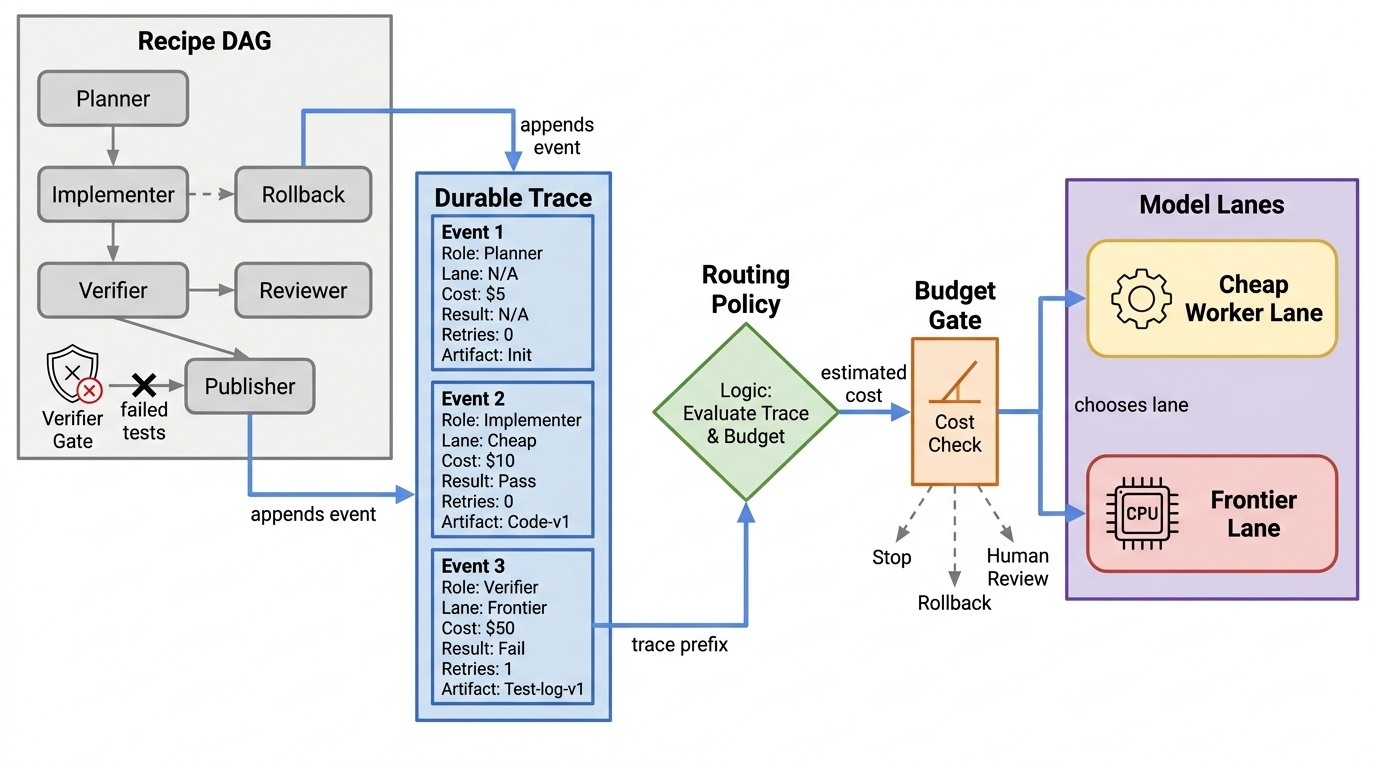
\includegraphics[width=0.96\linewidth]{assets/paperbanana-figures/trace-governed-paperbanana-v2.png}
\caption{Trace-governed budget allocation in mini-ork. A recipe DAG defines
roles and gates, each agent attempt appends events to the trace, and the next
routing decision uses the trace prefix, verifier state, and remaining budget.}
\label{fig:trace-loop}
\end{figure}

\section{Contributions}

This paper makes four contributions.

\begin{enumerate}
  \item We define trace-governed budget allocation, a policy class that maps
  workflow state, role labels, verifier outcomes, retry history, and remaining
  budget to model-lane choices.
  \item We model an agentic software workflow as a typed directed acyclic graph
  with planner, researcher, implementer, reviewer, verifier, reflector,
  publisher, and rollback nodes.
  \item Under explicit assumptions, we prove prefix budget boundedness,
  verifier-gated publication safety, monotone escalation, and cheap-first cost
  dominance under equal success.
  \item We provide a reproducible mini-ork experiment protocol and a controlled
  48-run benchmark comparing frontier-only, cheap-only, static role mapping,
  and trace-governed routing.
\end{enumerate}

\section{Related Work}

\paragraph{Budget-aware routing.}
MasRouter introduces multi-agent system routing over collaboration modes, role
allocation, and LLM selection \cite{masrouter2025}. Budget-aware agentic
routing frames routing as a sequential, path-dependent decision problem under
strict per-task budgets \cite{budgetaware2026}. ZEBRA allocates a fixed budget
across orchestration phases via an inference-time optimization formulation
\cite{zebra2026}. CASTER combines semantic and structural signals for
context-aware routing in graph-based multi-agent systems \cite{caster2026}.
xRouter trains a cost-aware orchestration system with reinforcement learning
\cite{xrouter2025}. These systems motivate the same economic problem as
mini-ork: not every step should receive the same model.

\paragraph{Adaptive orchestration.}
Difficulty-aware agentic orchestration generates query-specific workflows from
estimated difficulty \cite{daao2025}. Uno-Orchestra learns selective delegation
and worker choice \cite{unoorchestra2026}. AdaptOrch argues that orchestration
topology can matter more than individual model choice as model performance
converges \cite{adaptorch2026}. Flow treats workflows as activity-on-vertex
graphs that can be refined during execution \cite{flow2025}. mini-ork occupies
a complementary position: recipes define reusable workflows, while run traces
and gates provide dynamic control inside the workflow.

\paragraph{Verification and software-agent cost.}
Multi-Agent Verification studies scaling test-time compute with multiple
verifiers \cite{mav2025}. MAS-ProVe studies process verification in
multi-agent systems and reports substantial variance in current approaches
\cite{masprove2026}. FormalJudge explores neuro-symbolic oversight
\cite{formaljudge2026}, and AgentAuditor audits reasoning trees instead of
using simple majority vote \cite{agentauditor2026}. In software engineering,
AgentForge emphasizes execution-grounded verification \cite{agentforge2026},
Tokenomics quantifies where tokens are spent in agentic software workflows
\cite{tokenomics2026}, Co-Saving uses successful trajectories to reduce
resource use \cite{cosaving2025}, and trajectory reduction lowers cost by
removing redundant context \cite{agentdiet2025}. Retrieval-guided adaptive
orchestration connects topology selection to budget conservation
\cite{rgao2026}. mini-ork follows this broad line by treating deterministic
verifiers as first-class gates and traces as control inputs.

\section{System Model}

Let a workflow be a directed acyclic graph
\[
G=(V,E),
\]
where each node $v\in V$ has a type
\[
\tau(v) \in \{\text{planner}, \text{researcher}, \text{implementer},
\text{reviewer}, \text{verifier}, \text{reflector}, \text{publisher},
\text{rollback}\}.
\]
Each edge $e=(u,v)\in E$ has an edge type
\[
\epsilon(e)\in\{\text{depends\_on},\text{supplies\_context\_to},
\text{verifies},\text{blocks},\text{retries},\text{escalates\_to}\}.
\]

Let $M$ be the set of available model lanes. A lane is a symbolic role such as
\texttt{planner}, \texttt{worker}, \texttt{reviewer}, or a provider-specific
lens. Each lane resolves to a provider family through a configuration mapping
\[
\lambda:M\rightarrow P,
\]
where $P$ is the set of provider families.

A run trace after $t$ node attempts is
\[
H_t=\{h_1,h_2,\ldots,h_t\}.
\]
Each trace event $h_i$ contains at least
\[
h_i=(v_i,\tau(v_i),m_i,c_i,r_i,g_i,a_i),
\]
where $v_i$ is the node, $m_i$ is the selected model lane, $c_i\ge 0$ is cost,
$r_i$ is runtime, $g_i$ is the verifier or gate outcome, and $a_i$ is an
artifact reference. The cumulative cost at time $t$ is
\[
C(H_t)=\sum_{i=1}^{t}c_i.
\]
The workflow has a budget $B>0$. A valid run must satisfy
\[
C(H_t)\le B
\]
for every prefix $H_t$.

\section{Trace-Governed Budget Allocation}

A trace-governed budget allocation policy is a function
\[
\pi(v,H_t,B)\rightarrow m
\]
that chooses a model lane $m\in M$ for the next node attempt. The policy may
inspect the node type $\tau(v)$, previous verifier outcomes in $H_t$, retry
count for node $v$, remaining budget $B-C(H_t)$, artifact risk class,
model-lane cost profile, and confidence or severity of reviewer feedback. It
must not inspect hidden state from future nodes; decisions are online and use
only the trace prefix.

\subsection{Policy Skeleton}

A simple trace-governed policy has four rules.

\begin{enumerate}
  \item \textbf{Cheap-first implementation.} Use a low-cost worker lane for
  bounded implementer tasks while no verifier has failed.
  \item \textbf{Frontier planning and recovery.} Use a frontier lane for
  planning and for recovery after verifier failure, repeated retries, or
  high-risk artifact changes.
  \item \textbf{Verifier-gated continuation.} Do not run publisher nodes unless
  required verifier gates pass.
  \item \textbf{Budget stop.} If the next selected lane would exceed the
  remaining budget, stop, rollback, or escalate to a human gate.
\end{enumerate}

\subsection{Risk-Weighted Escalation Score}

Let the escalation score for a node be
\[
S(v,H_t)=\alpha R(v)+\beta F(v,H_t)+\gamma K(v,H_t)+\delta U(v,H_t),
\]
where $R(v)$ is the static risk score of the artifact touched by $v$,
$F(v,H_t)$ is the number or severity of failed verifier events relevant to
$v$, $K(v,H_t)$ is the retry count for $v$, $U(v,H_t)$ is uncertainty from
reviewer disagreement or missing evidence, and
$\alpha,\beta,\gamma,\delta\ge 0$. For threshold $\theta$, the policy selects a
frontier lane when
\[
S(v,H_t)\ge\theta
\]
and a cheaper lane otherwise, subject to the budget constraint.

\begin{figure}[t]
\centering
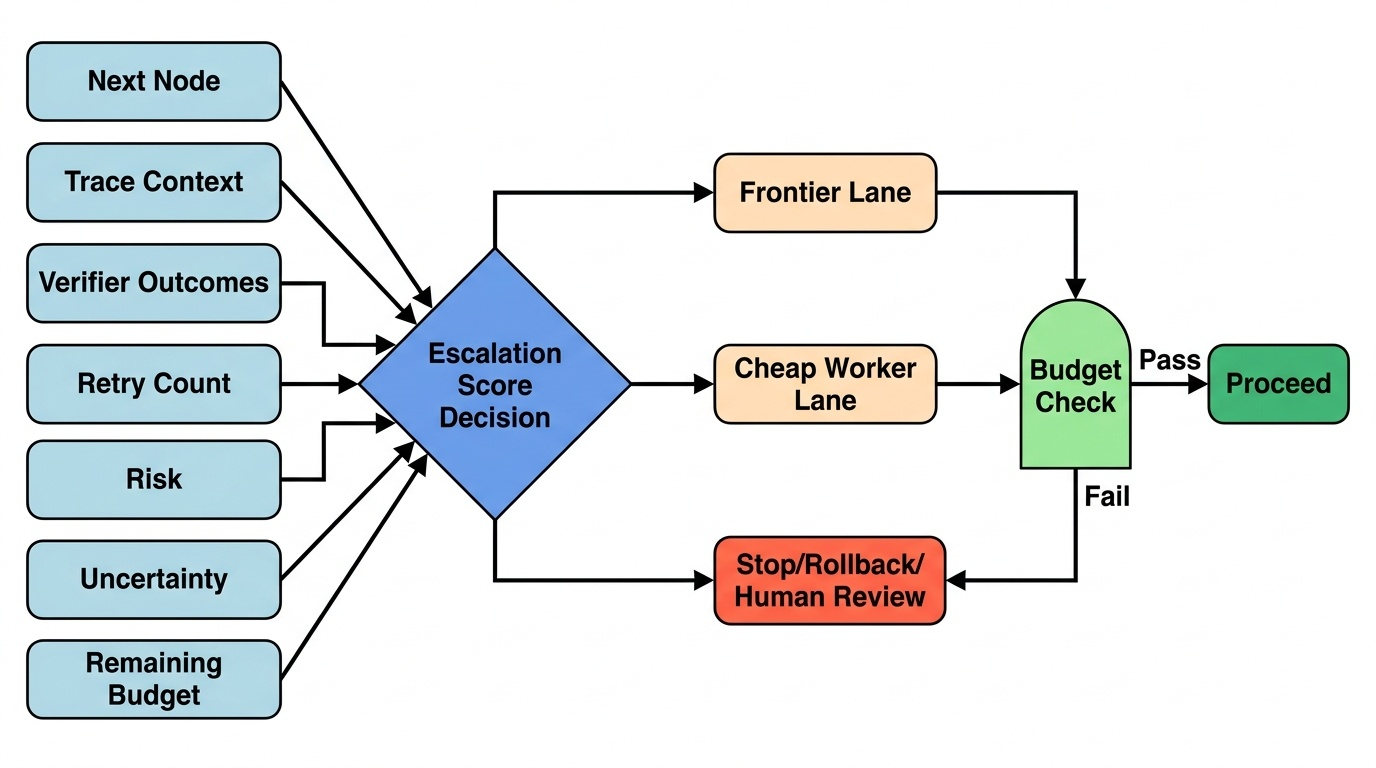
\includegraphics[width=0.96\linewidth]{assets/paperbanana-figures/policy-decision-paperbanana.png}
\caption{Decision structure for a simple trace-governed policy. Clean
implementation nodes can use cheap lanes, while failed verifiers, retries,
uncertainty, high risk, or budget pressure trigger escalation, rollback, or a
human gate.}
\label{fig:policy-decision}
\end{figure}

\section{Formal Properties}

The following propositions establish basic safety properties of the policy
class. They prove what the budget governor can guarantee by construction, not
that every task outcome will be semantically correct.

\begin{proposition}[Prefix budget boundedness]
Let $B>0$ be the run budget. Suppose policy $\pi$ selects a lane for node
$v_{t+1}$ only if the estimated maximum cost of the next attempt,
$\widehat{c}_{t+1}$, satisfies
\[
C(H_t)+\widehat{c}_{t+1}\le B.
\]
Assume actual cost is bounded by the estimate:
\[
c_{t+1}\le \widehat{c}_{t+1}.
\]
Then every trace prefix produced by $\pi$ satisfies $C(H_t)\le B$.
\end{proposition}

\begin{proof}
We prove by induction on $t$. For $t=0$, $C(H_0)=0\le B$. Assume
$C(H_t)\le B$. The policy permits the next attempt only when
$C(H_t)+\widehat{c}_{t+1}\le B$. Since
$c_{t+1}\le\widehat{c}_{t+1}$, we have
\[
C(H_{t+1})=C(H_t)+c_{t+1}
\le C(H_t)+\widehat{c}_{t+1}
\le B.
\]
Thus the invariant holds for $t+1$. By induction, all prefixes are
budget-bounded.
\end{proof}

\begin{proposition}[Verifier-gated publication safety]
Let $p$ be a publisher node. Suppose every path to $p$ contains a verifier node
$q$ with an edge type \texttt{verifies}, and suppose the executor blocks $p$
unless $q$'s latest gate result is pass. Then no artifact is published from a
run whose required verifier failed or is absent.
\end{proposition}

\begin{proof}
By construction, $p$ is reachable only after its predecessor requirements are
satisfied. Since every path to $p$ contains a verifier gate $q$, and the
executor blocks $p$ unless $q$ has a pass result, any run that reaches $p$ must
contain a passing result for each required verifier. If a verifier failed or
did not run, the precondition for $p$ is false, so $p$ cannot execute.
\end{proof}

\begin{proposition}[Monotone escalation]
Assume the escalation score is
\[
S(v,H_t)=\alpha R(v)+\beta F(v,H_t)+\gamma K(v,H_t)+\delta U(v,H_t)
\]
with nonnegative coefficients. If a trace extension increases any of $F$, $K$,
or $U$ and leaves all other terms unchanged, then $S(v,H_t)$ does not decrease.
\end{proposition}

\begin{proof}
Let $H_{t'}$ be a trace extension of $H_t$. Suppose one or more of $F$, $K$, or
$U$ increases, no term decreases, and $\alpha,\beta,\gamma,\delta\ge 0$. Then
$S(v,H_{t'})-S(v,H_t)$ is a sum of nonnegative coefficients multiplied by
nonnegative term differences. The result is nonnegative.
\end{proof}

\begin{proposition}[Cheap-first dominance under equal success]
Consider two policies over the same workflow prefix: a frontier-only policy
$\pi_f$ and a cheap-first policy $\pi_c$. Suppose for each implementation node
before the first verifier failure, both policies have equal probability of
eventual verifier pass, and the cheap lane has cost no greater than the
frontier lane. Then the expected cost of $\pi_c$ before the first verifier
failure is no greater than that of $\pi_f$.
\end{proposition}

\begin{proof}
Over the prefix before the first verifier failure, both policies execute the
same set of implementation nodes by assumption. For each such node $v_i$, let
the frontier cost be $c_f(v_i)$ and the cheap cost be $c_c(v_i)$, with
$c_c(v_i)\le c_f(v_i)$. The expected prefix cost is the sum of node costs
weighted by the probability that the node is reached. The reach probabilities
are equal because the policies have equal pass probability over the prefix by
assumption. Therefore each weighted term for $\pi_c$ is no larger than the
corresponding term for $\pi_f$, and the total expected cost is no larger.
\end{proof}

\section{Implementation in mini-ork}

mini-ork implements the abstractions required by the formal model. Workflow
nodes reference symbolic lanes rather than concrete vendor models. A recipe can
preserve its role structure while the operator changes provider families
according to price, availability, or experimental condition. The state database
records run lifecycle, task runs, execution traces, model costs, artifacts,
gate results, gradients, workflow candidates, benchmark results, and promotion
decisions. Recipes can also ship executable verifier scripts such as tests,
typechecks, schema checks, lint, migration replay, or artifact-shape
validation. Verifier output is a control signal for the policy, not merely an
audit log.

\section{Experimental Protocol}

The empirical question is whether trace-governed routing lowers cost per
successful task without reducing correctness.

\subsection{Task Suites and Baselines}

The benchmark contains three task classes: \texttt{obs\_smoke},
\texttt{docs}, and \texttt{code\_fix}. \texttt{obs\_smoke} tasks exercise a
small live LLM workflow; \texttt{docs} tasks require deterministic
documentation edits with grep-based checks; \texttt{code\_fix} tasks require
repairing small Python fixtures with typecheck and test verifiers.

We compare four policies: frontier-only, cheap-only, static role mapping, and
trace-governed routing. Frontier-only routes every model-executed node to the
expensive lane. Cheap-only routes every model-executed node to the cheap lane.
Static role mapping assigns planner and reviewer roles to frontier lanes and
implementation roles to cheap lanes, without trace-dependent escalation.
Trace-governed routing uses trace prefix, verifier outcomes, retry count, role,
and budget state to route each next attempt. A query-level workflow-generation
baseline remains future work.

\subsection{Metrics}

The primary metric is cost per successful task:
\[
\text{Cost per successful task}
=
\frac{\text{total cost across runs}}{\text{number of successful runs}}.
\]
We also report deterministic verifier pass rate, reviewer accept rate,
wall-clock duration, expensive model calls, retries, and plan fallback count.

\subsection{Hypotheses}

\begin{description}
  \item[H1] Trace-governed routing reduces cost per successful task relative to
  frontier-only routing.
  \item[H2] Trace-governed routing improves success rate relative to cheap-only
  routing.
  \item[H3] Trace-governed routing reduces unnecessary frontier-model calls
  relative to static role mapping when verifier outcomes are clean.
  \item[H4] Trace-governed routing reduces repeated failed cheap-model attempts
  relative to static role mapping when verifier failures accumulate.
\end{description}

\section{Controlled Benchmark}

We ran a controlled mini-ork benchmark on 2026-06-10 and 2026-06-11. Each
policy was evaluated on 12 live LLM runs, for 48 total runs. All runs reached
\texttt{published} status and all deterministic verifier checks passed.

\begin{figure}[t]
\centering
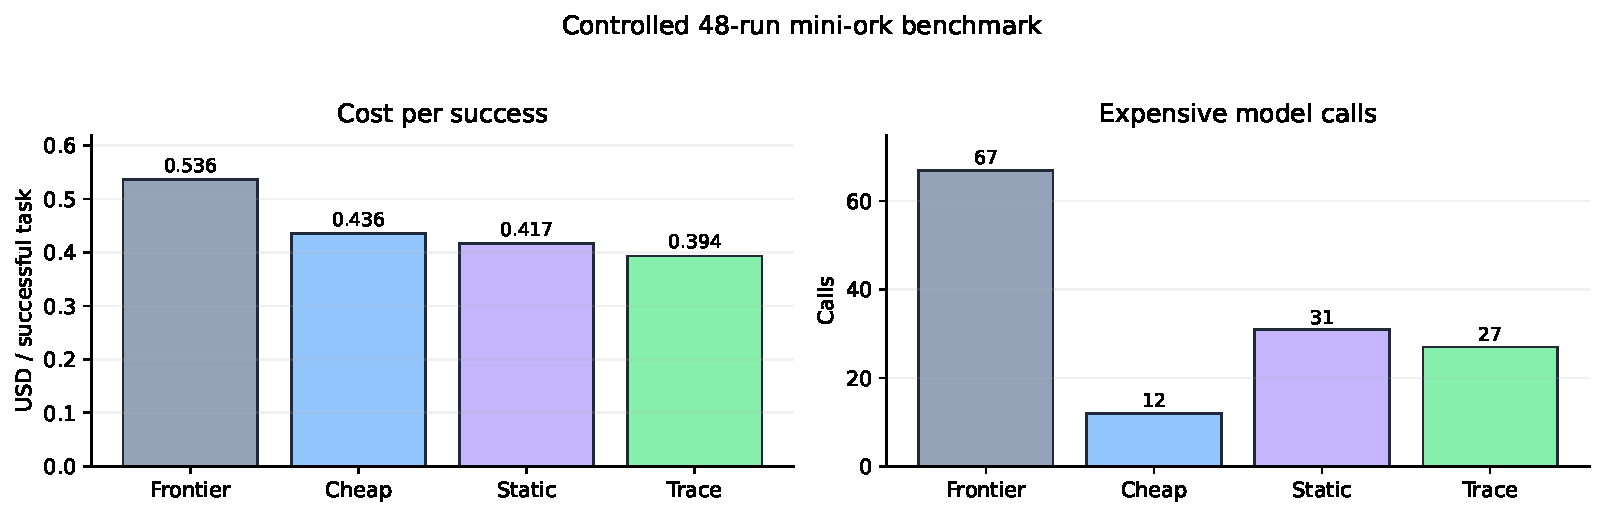
\includegraphics[width=0.92\linewidth]{assets/deterministic-figures/benchmark_cost_calls.pdf}
\caption{Cost and expensive-call comparison for the controlled 48-run
benchmark. Trace-governed routing preserves the observed verifier pass rate
while reducing both cost per success and expensive model calls relative to
frontier-only routing.}
\label{fig:benchmark-cost}
\end{figure}

\begin{table}[t]
\centering
\caption{Controlled mini-ork benchmark across three task classes. Cost is in
USD as recorded by the mini-ork run ledger.}
\label{tab:benchmark}
\small
\setlength{\tabcolsep}{3.5pt}
\begin{tabular}{lrrrrrrr}
\toprule
Policy & Runs & Succ. & Verif. & Rev. & Cost/succ. & Med. s & Exp. calls \\
\midrule
Frontier-only & 12 & 1.000 & 1.000 & 0.889 & 0.536418 & 87.0 & 67 \\
Cheap-only & 12 & 1.000 & 1.000 & 1.000 & 0.435822 & 132.0 & 12 \\
Static role mapping & 12 & 1.000 & 1.000 & 0.889 & 0.416641 & 93.0 & 31 \\
Trace-governed & 12 & 1.000 & 1.000 & 0.889 & 0.393587 & 99.0 & 27 \\
\bottomrule
\end{tabular}
\end{table}

Trace-governed routing reduced cost per successful task by 26.63\% versus
frontier-only routing with no observed verifier-pass loss. It also reduced
expensive model calls from 67 to 27 across the benchmark. Relative to static
role mapping, trace-governed routing reduced cost per successful task by 5.53\%
and reduced expensive calls from 31 to 27. The Wilson 95\% interval for each
12/12 verifier pass rate is $[0.7575,1.0]$.

This result supports the narrow benchmark claim: on these controlled mini-ork
fixtures, trace-governed routing reduced cost relative to frontier-only routing
while preserving deterministic verifier pass rate. It does not prove that cheap
models can replace frontier models in arbitrary production work. The fixtures
are small, the query-level workflow baseline has not yet been implemented, and
reviewer acceptance was not perfect for code-fix runs.

\section{Threats to Validity}

\paragraph{Provider drift.}
Hosted model behavior and pricing change over time. Evaluation must record
provider, model, date, and price assumptions.

\paragraph{Task leakage.}
Repository tasks may be easier for models that have seen similar public code.
The benchmark should include private or freshly generated tasks where possible.

\paragraph{Verifier incompleteness.}
Passing tests or typecheck does not prove semantic correctness. This is a
limitation of execution-grounded software-agent benchmarks.

\paragraph{Fixture ceiling effects.}
The controlled benchmark uses small deterministic fixtures. A 100\% verifier
pass rate across all policies means the current benchmark primarily
distinguishes cost and routing behavior, not hard-task reliability.

\paragraph{Planner fallback contamination.}
In the \texttt{obs\_smoke} portion of the benchmark, some runs used
deterministic fallback planning after the planner emitted invalid JSON. This
preserves the run but weakens any claim about whole-run model routing. Future
batches should route planner calls through the policy surface or report planner
fallback as a separate framework failure mode.

\paragraph{Reviewer variance.}
Reviewer labels are useful but noisy; future batches should blind reviewers to
policy labels or use deterministic reviewer evidence contracts.

\section{Discussion}

Trace-governed budget allocation reframes observability as a control surface.
Instead of treating agent traces as logs for debugging after a run completes,
the workflow uses the trace prefix to decide how much reasoning power the next
step deserves. A cheap worker that passes a deterministic verifier should not
be replaced by a frontier model merely because the workflow is important.
Conversely, a cheap worker that repeatedly fails the same verifier should not
be allowed to burn budget indefinitely.

The approach is compatible with adaptive-orchestration work. Query-level
workflow generation decides the shape of the run before execution.
Trace-governed routing decides resource allocation during execution. These are
complementary: a generated workflow can still use trace-governed budget
allocation inside the workflow.

\section{Conclusion}

We introduced trace-governed budget allocation for heterogeneous multi-agent
LLM software workflows. The central idea is simple: persistent execution traces
should govern future inference spend. We formalized workflows as typed DAGs,
defined an online routing policy over trace prefixes, proved budget and
verifier-gating properties, and reported a controlled 48-run benchmark.

The benchmark supports the claim that trace-governed routing can reduce cost
relative to frontier-only routing on small verifier-gated mini-ork tasks while
preserving deterministic verifier pass rate. The next step is to scale the
benchmark to harder tasks, implement the query-level workflow baseline, and add
blinded human-review labels.

\section*{Data and Code Availability}

The implementation is in the mini-ork repository. Experiment manifests and
results used in this paper are stored under the repository path
\texttt{docs/research/experiments/}. The key result directory is named
\texttt{trace-budget-cross-task-20260611-48}. The analyzer is in
\texttt{scripts/research/}; the routing policy implementation is in
\texttt{bin/mini-ork-execute}.

\appendix

\section{Reproducibility Notes}

The controlled result can be regenerated with the mini-ork CLI and the research
scripts in this repository. The high-level flow is:
\begin{enumerate}
  \item Run the observation-smoke batch script.
  \item Run the fixture batch script for documentation and code-fix tasks.
  \item Analyze both manifests into the combined cross-task result directory.
\end{enumerate}
The exact checked-in outputs are retained so the paper table is auditable even
when provider prices or model behavior drift.

\section{Minimal Routing Pseudocode}

\begin{verbatim}
function route(node, trace, budget):
    remaining = budget - cost(trace)
    score = risk(node)
          + failed_verifiers(node, trace)
          + retry_count(node, trace)
          + uncertainty(node, trace)

    if next_attempt_exceeds_budget(node, remaining):
        return HUMAN_GATE_OR_ROLLBACK

    if node.type in {planner, reviewer}:
        return FRONTIER_LANE

    if score >= ESCALATION_THRESHOLD:
        return FRONTIER_LANE

    return CHEAP_WORKER_LANE
\end{verbatim}

\bibliographystyle{plain}
\bibliography{references}

\end{document}
